\documentclass{lab_sheet}
\usepackage{pgfplots}
\usepackage{tikz}
\usepackage{wrapfig}
\usetikzlibrary{decorations.pathreplacing}
\pgfplotsset{compat=newest}
\begin{document}
    \titlePage{Amplitude Modulation}{February 8, 2021}
    \pagenumbering{gobble}
    \tableofcontents
    \pagebreak
    \pagenumbering{arabic}
    \section{Objectives}
    \begin{itemize}
        \item Understanding the properties of double side band (DSB), double side band with full carrier (DSB-FC) and double side band with suppressed carrier (DSB-SC)
    \end{itemize}
    \section{Required Tools}
    \begin{itemize}
        \item Signal generator
        \item Double beam digital oscilloscope
        \item ED-2900P, ED-2950D and ED-2960D
        \item Signal processing and wireless communications MATLAB application modules
    \end{itemize}
\section{Introduction}
For a signal to communicate over a channel, it is important to be able to vary one of the parameters of a high frequnecy signal with respect to the actual signal that represents the information that we are trying to communicate. 
\subsection{Message Signal}
Message signal is a low frequnecy signal that serves as the true message to communicate over a channel. It is also known as modulating signal since the amplitude of the carrier signal varies in accordance with the message signal. Figure~\ref{fig:msg} shows the message signal as $m(t)=A_m cos(2\pi f_m t)$.
    \begin{figure}[H]
        \centering
        \begin{tikzpicture}
            \begin{axis}[
                xlabel={Time},
               ylabel={Amplitude},
                axis lines=center,
                axis x line=center,
                axis y line=center,
                ymin=-5.5,
                ymax=5.5,
                xmin=-1,
                xlabel style={below right},
                ylabel style={left},
                xtick=\empty, ytick=\empty
            ]
               \draw [decorate,decoration={brace,raise=2pt}]
(0,0) -- (0,2) node [black,midway,xshift=-6pt, left] {
$A_m$};
              \addplot[domain=0:2*pi,black,samples=501] {2*cos(x*2*180/pi)};
            \end{axis}
          \end{tikzpicture} 
          \caption{Message signal}
          \label{fig:msg}
    \end{figure}

\subsection{Carrier Signal}
Carrier signal is a high frequnecy signal that essentially has no information associated with its amplitude. It varies its amplitude during modulation in accordance with the instantaneous amplitude of the modulating signal. Figure~\ref{fig:car} shows the carrier signal as $c(t)=A_c cos(2\pi f_c t)$.
    \begin{figure}[H]
        \centering
        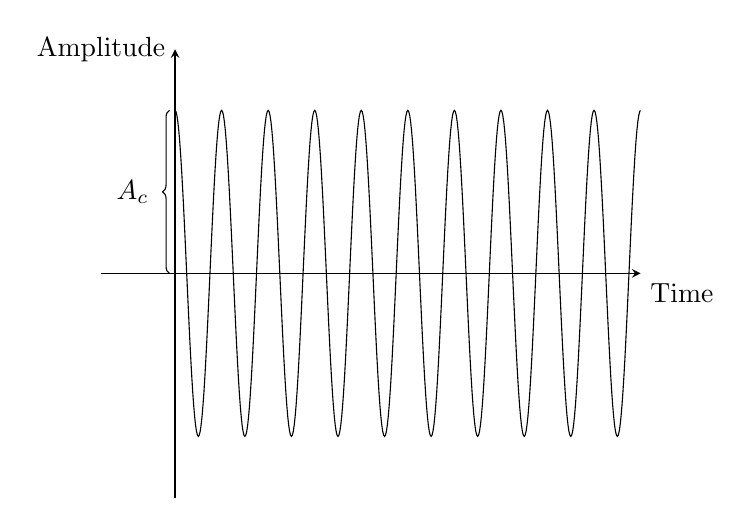
\begin{tikzpicture}
            \begin{axis}[
                xlabel={Time},
                ylabel={Amplitude},
                axis lines=center,
                axis x line=center,
                axis y line=center,
                ymin=-5.5,
                ymax=5.5,
                xmin=-1,
                xlabel style={below right},
                ylabel style={left},
                xtick=\empty, ytick=\empty
            ]
               \draw [decorate,decoration={brace,raise=2pt}]
(0,0) -- (0,4) node [black,midway,xshift=-6pt, left] {
$A_c$};
              \addplot[domain=0:2*pi,black,samples=501] {4*cos(5*x*2*180/pi)};
            \end{axis}
          \end{tikzpicture} 
          \caption{Carrier signal}
          \label{fig:car}
    \end{figure}

    \subsection{Amplitude Modulated Signal}
    Amplitude modulated signal is actually the carrier signal whose one or more parameters are varied according to the modulating signal. Figure~\ref{fig:amp} shows the modulated signal as $s(t)=[A_c + A_m cos(2\pi f_m t)]cos(2\pi f_c t)$. It is to be noted that there is an envelope structure signal that bounds the carrier wave and is in fact the modulating wave hence giving rise to the modulated signal.
    \begin{figure}[H]
        \centering
        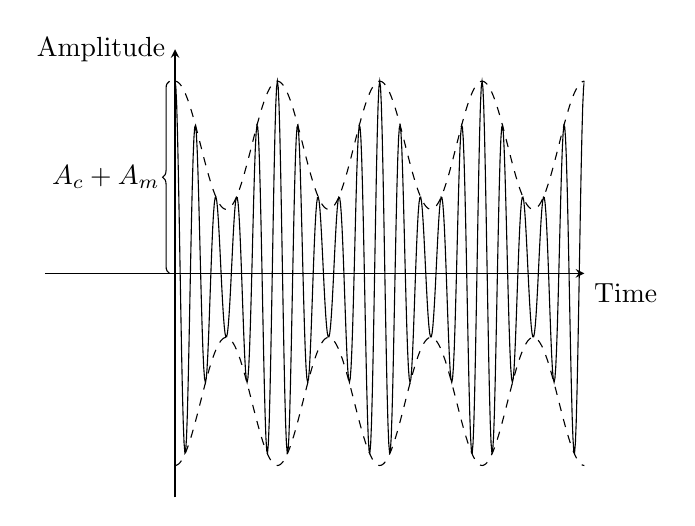
\begin{tikzpicture}
            \begin{axis}[
                xlabel={Time},
                ylabel={Amplitude},
                axis lines=center,
                axis x line=center,
                axis y line=center,
                ymin=-7,
                ymax=7,
                xmin=-4,
                xlabel style={below right},
                ylabel style={left},
                xtick=\empty, ytick=\empty
            ]
               \draw [decorate,decoration={brace,raise=2pt}]
(0,0) -- (0,6) node [black,midway,xshift=-25pt] {
$A_c+A_m$};
\addplot[domain=0:4*pi,black,samples=501,dashed] {4+2*cos(x*2*180/pi)};
\addplot[domain=0:4*pi,black,samples=501,dashed] {-4-2*cos(x*2*180/pi)};
              \addplot[domain=0:4*pi,black,samples=501] {(4+2*cos(x*2*180/pi))*cos(5*x*2*180/pi)};
            \end{axis}
          \end{tikzpicture} 
          \caption{Amplitude modulated signal}
          \label{fig:amp}
    \end{figure}

    \subsection{Modulation Index}
    Modulation index or modulation depth is the ratio of change in the amplitude of carrier signal to the amplitude of carrier signal. It identifies the level of modulation that a carrier signal undergoes. It is often represented as percentage of modulation which is calculated by multiplying the ratio by 100. 
    \subsubsection*{Derivation}
    If we consider the message signal as,
    $$
    m(t)=A_m cos(2\pi f_m t)
    $$
    and the carrier signal as,
    $$
    c(t)=A_c cos(2\pi f_c t)
    $$
    where, \\
    $A_m$ and $f_m$ are the amplitude and frequency of the message signal and $A_c$ and $f_c$ are the amplitude and frequency of the carrier signal. \\
    As mentioned earlier, the modulated signal will have the equation as,
    \begin{equation*}
        \begin{aligned}
            s(t)&=[A_c + A_m cos(2\pi f_m t)]cos(2\pi f_c t)\\
            &=A_c[1 + \frac{A_m}{A_c} cos(2\pi f_m t)]cos(2\pi f_c t)\\
            &=A_c[1 + \mu cos(2\pi f_m t)]cos(2\pi f_c t)
        \end{aligned}
    \end{equation*}
    where, \\
    $\mu$ is the modulation index given as,
    $$\mu=\frac{A_m}{A_c}$$
    If the amplitudes of message and carrier signal are unknown, then the modulation index can be calculated as,
    $$
    \mu = \frac{A_{max}-A_{min}}{A_{max}+A_{min}}
    $$
    \subsubsection{Under Modulation}
    If the value of modulation index is less than 1, the modulation is called under modulation and the modulated result is called under-modulated signal.
    \begin{figure}[H]
        \centering
        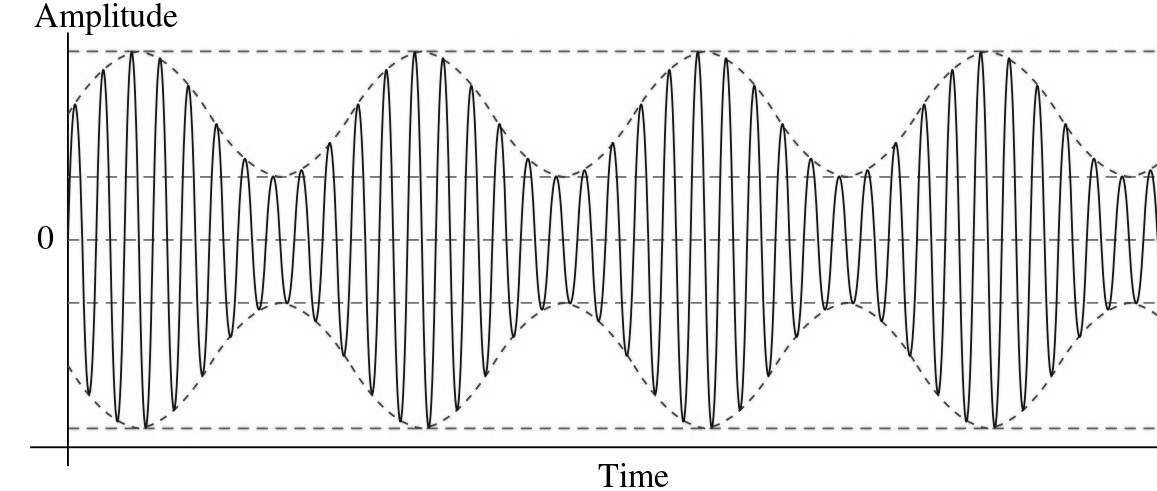
\includegraphics[width=.95\linewidth]{./Figures/under.png}
        \caption{Under-modulated signal}
        \label{fig:under}
    \end{figure}
    \subsubsection{Perfect Modulation}
    If the value of modulation index is equal to 1, the modulation is called perfect modulation and the modulated result is called perfectly-modulated signal.
    \begin{figure}[H]
        \centering
        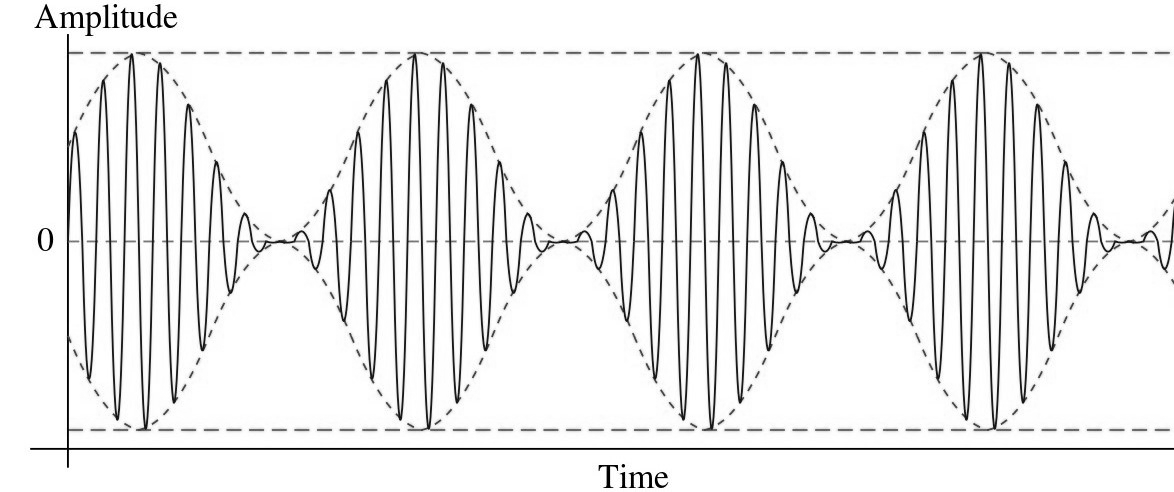
\includegraphics[width=.95\linewidth]{./Figures/perfect.png}
        \caption{Perfectly-modulated signal: 100\% modulated signal}
        \label{fig:perfect}
    \end{figure}
    \subsubsection{Over Modulation}
    If the value of modulation index more than 1, the modulation is called over modulation and the modulated result is called over-modulated signal.
    \begin{figure}[H]
        \centering
        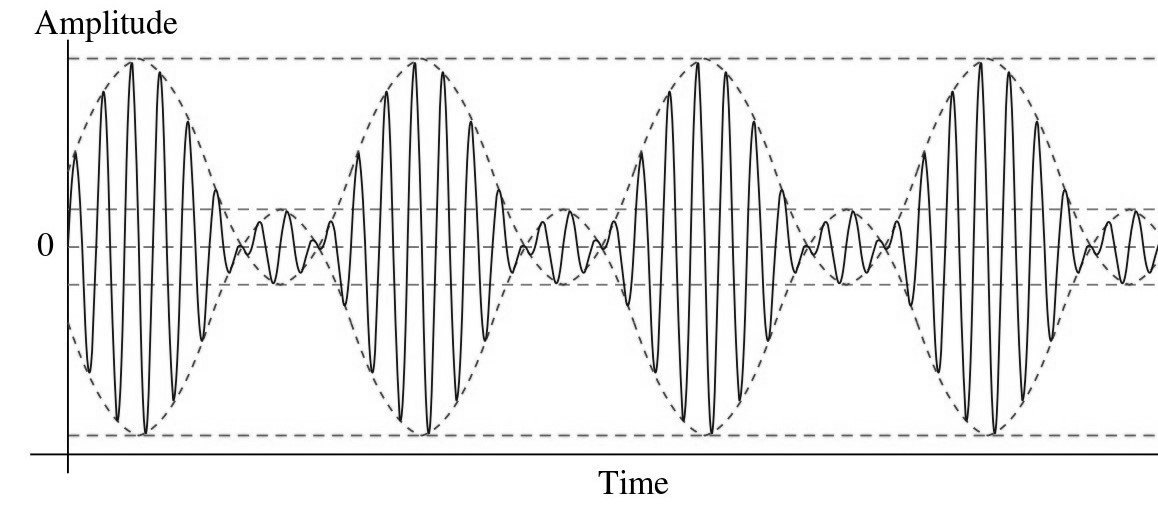
\includegraphics[width=.95\linewidth]{./Figures/over.png}
        \caption{Over-modulated signal}
        \label{fig:over}
    \end{figure}
    \subsection{DSB-FC and DSB-SC}
    Double side band- full carrier (DSB-FC) means that the resulting amplitude modulated signal generated will always contain the carrier component along with the combination of the message and carrier signal. It essentially means that there is an additional carrier component along with the multiplication of message and carrier signals.\\
    Since the carrier signal contains no true information, the transmission of such signal is a waste of power. Amplitude modulation is in fact a high bandwidth consumer as unrequired double side bands are transmitted when only one side band is enough for transmission of the data. Thus there is a need to suppress the carrier signal and hence modify the sidebands of the modulated wave. Double side band- suppressed carrier (DSB-SC) means that the carrier part will be removed from the modulated signal hence only transmitting the combination of message and carrier signals. DSB-SC is useful to ensure the discrete carrier signal is suppressed. 
    \section{Lab Experiment Observations}
    Modulating signal frequency ($f_m$) = 50 Hz\\
    Carrier signal frequency ($f_c$) = 955 Hz 
    
    \subsection*{Under Modulation}
    \begin{figure}[H]
     \centering
            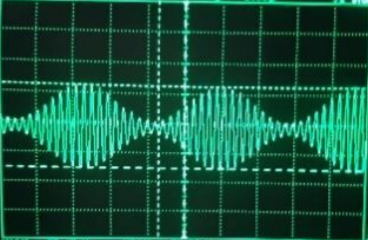
\includegraphics[scale=0.8]{Figures/dsb_fc_under.png}
        \caption{AM signal for under modulation}
      \end{figure}
      \begin{align*}
       A_{max}&=7.03~V\\
       A_{min}&=1.33~V\\
       \mu&=\frac{A_{max}-A_{min}}{A_{max}+A_{min}}=0.6818
      \end{align*}

      \subsection*{Perfect Modulation}
      \begin{figure}[H]
        \centering
               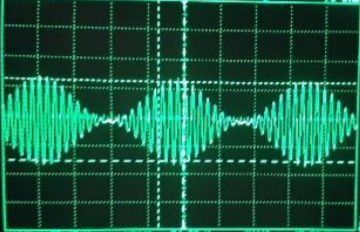
\includegraphics[scale=0.8]{Figures/dsb_fc_perfect.png}
           \caption{AM signal for perfect modulation}
         \end{figure}
         \begin{align*}
          A_{max}&=9.14~V\\
          A_{min}&=0~V\\
          \mu&=\frac{A_{max}-A_{min}}{A_{max}+A_{min}}=1
         \end{align*}

         \subsection*{Over Modulation}
         \begin{figure}[H]
           \centering
                  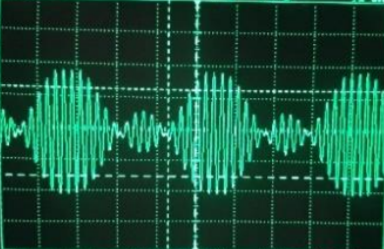
\includegraphics[scale=0.8]{Figures/dsb_fc_over.png}
              \caption{AM signal for over modulation}
            \end{figure}
            \begin{align*}
             A_{max}&=9.85~V\\
             A_{min}&=-3.67~V\\
             \mu&=\frac{A_{max}-A_{min}}{A_{max}+A_{min}}=2.1877
            \end{align*}

\section{MATLAB Scripts}
\subsection{DSB-FC Generation}
The modulation index $\mu$ is represented by the variable $m$, which is a user prompt input that can be used to plot AM signals for different modulation indices.
\matlabcode{dsb_fc}{DSB-FC Generation}

\subsection{DSB-SC Generation}
\matlabcode{dsb_sc}{DSB-SC Generation}

\section{Simulated Signal Observations}
The values of modulation index $m$ have been chosen as 0.6818, 1 and, 2.1877, which were the obtained results from the actual lab experiment. 
\subsection{DSB-FC}
\subsection*{Under Modulation (For m = 0.6818)}
\begin{figure}[H]
 \centering
        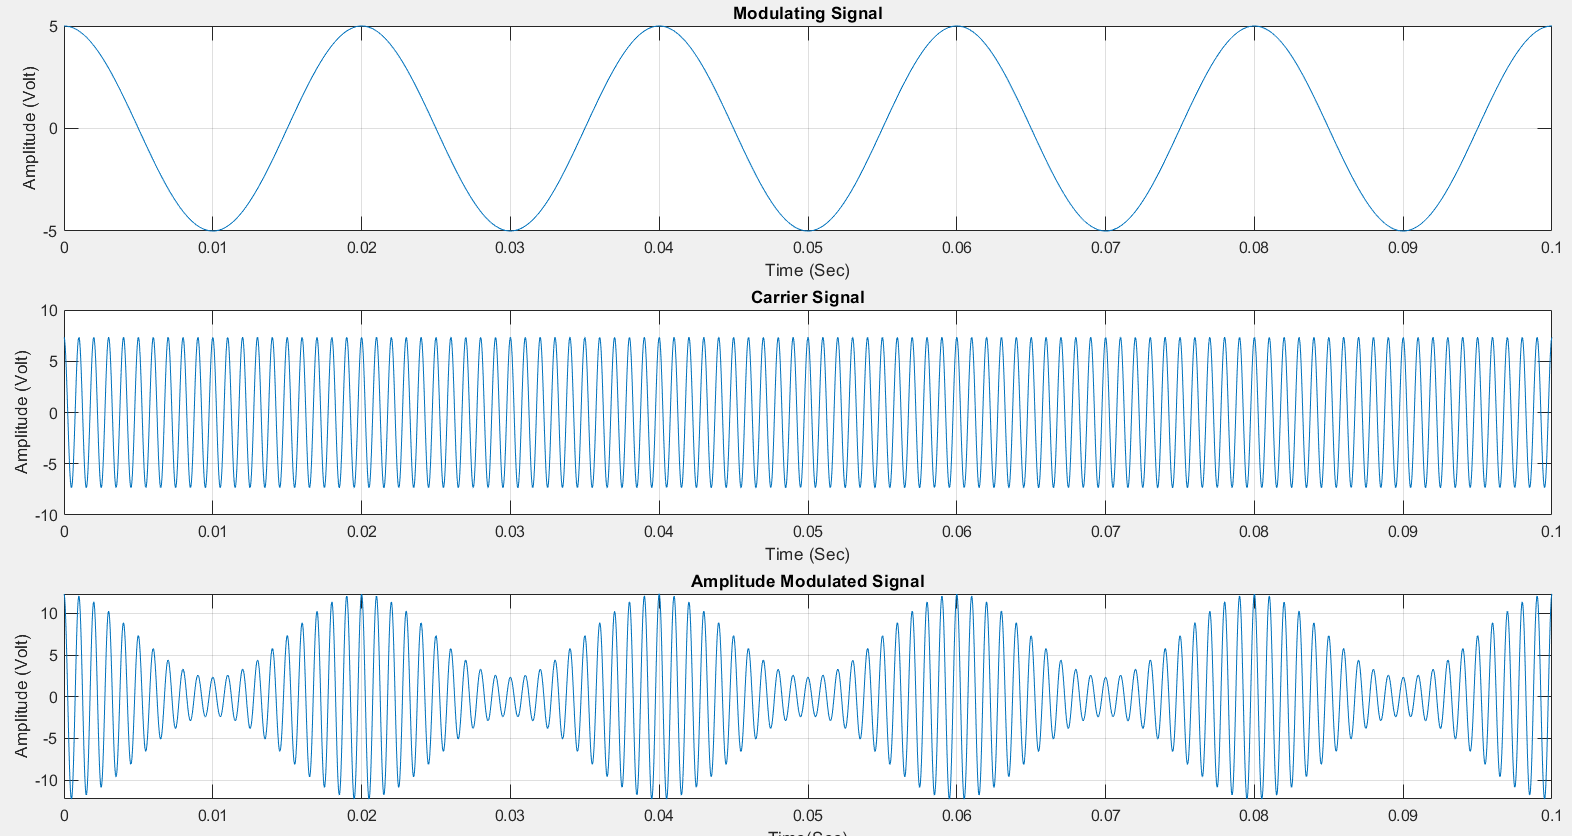
\includegraphics[width=.9\linewidth]{Figures/sim_dsb_fc_under.png}
    \caption{Simulated AM signal for under modulation}
  \end{figure}

  \subsection*{Perfect Modulation (For m = 1)}
  \begin{figure}[H]
    \centering
           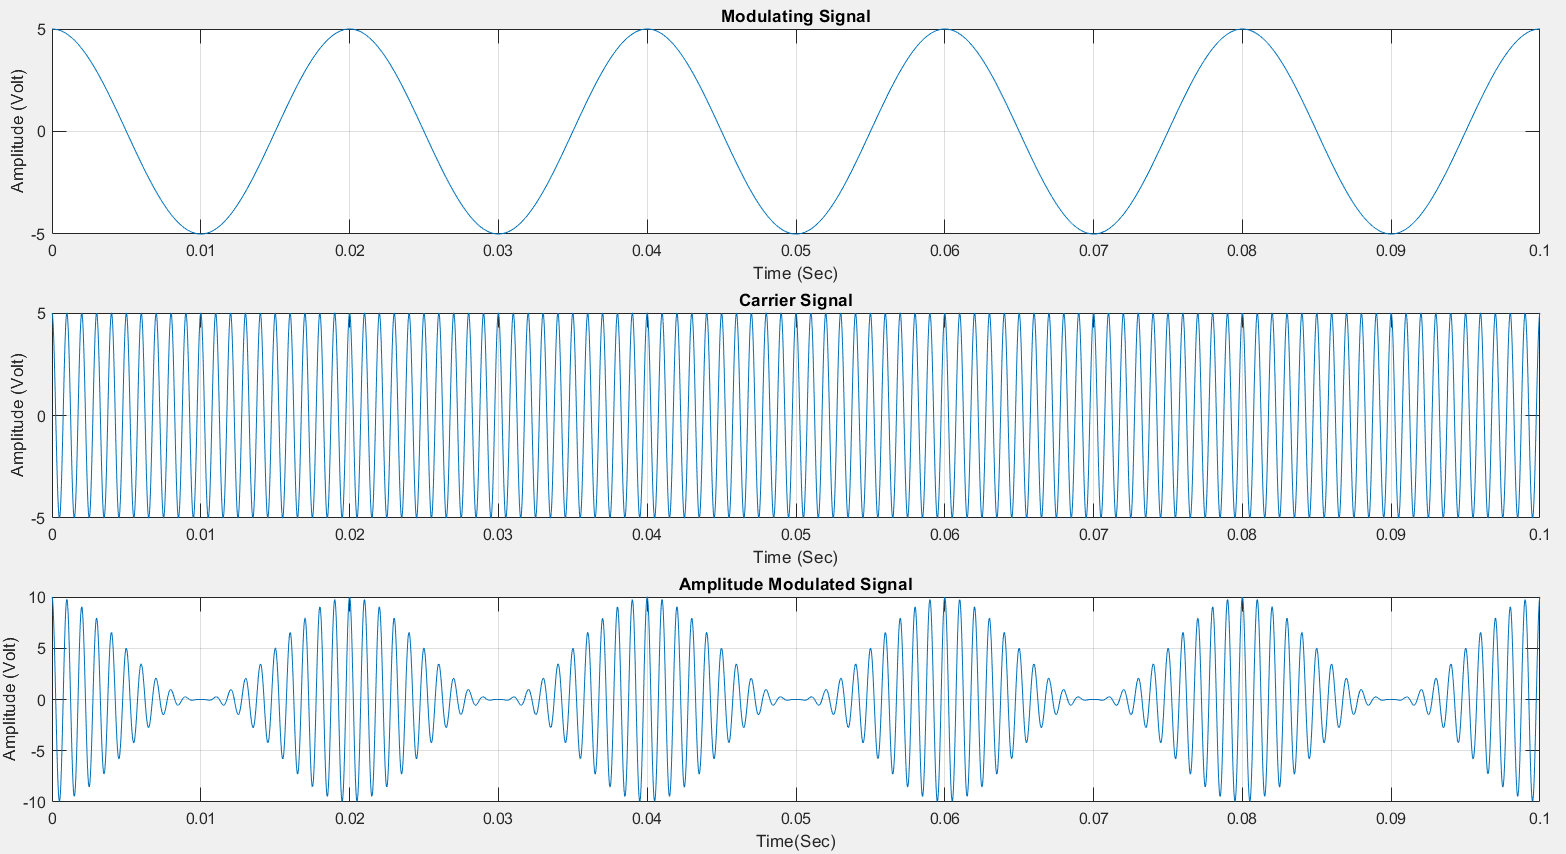
\includegraphics[width=.9\linewidth]{Figures/sim_dsb_fc_perfect.png}
       \caption{Simulated AM signal for perfect modulation}
     \end{figure}

     \subsection*{Over Modulation (For m = 2.1877)}
     \begin{figure}[H]
       \centering
              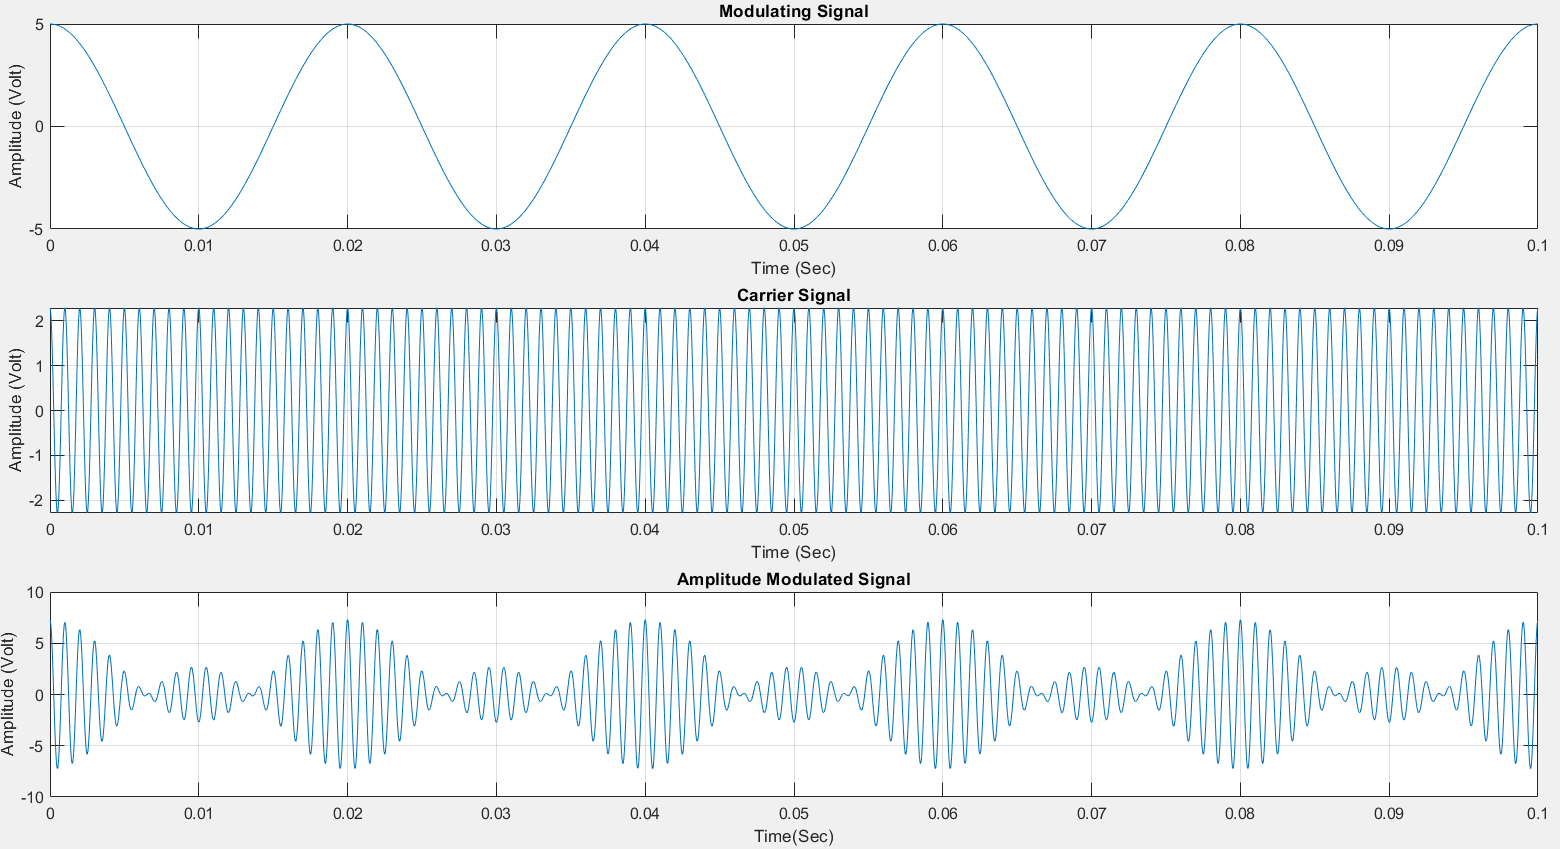
\includegraphics[width=.9\linewidth]{Figures/sim_dsb_fc_over.png}
          \caption{Simulated AM signal for over modulation}
        \end{figure}
        \subsection{DSB-SC}
     \begin{figure}[H]
       \centering
              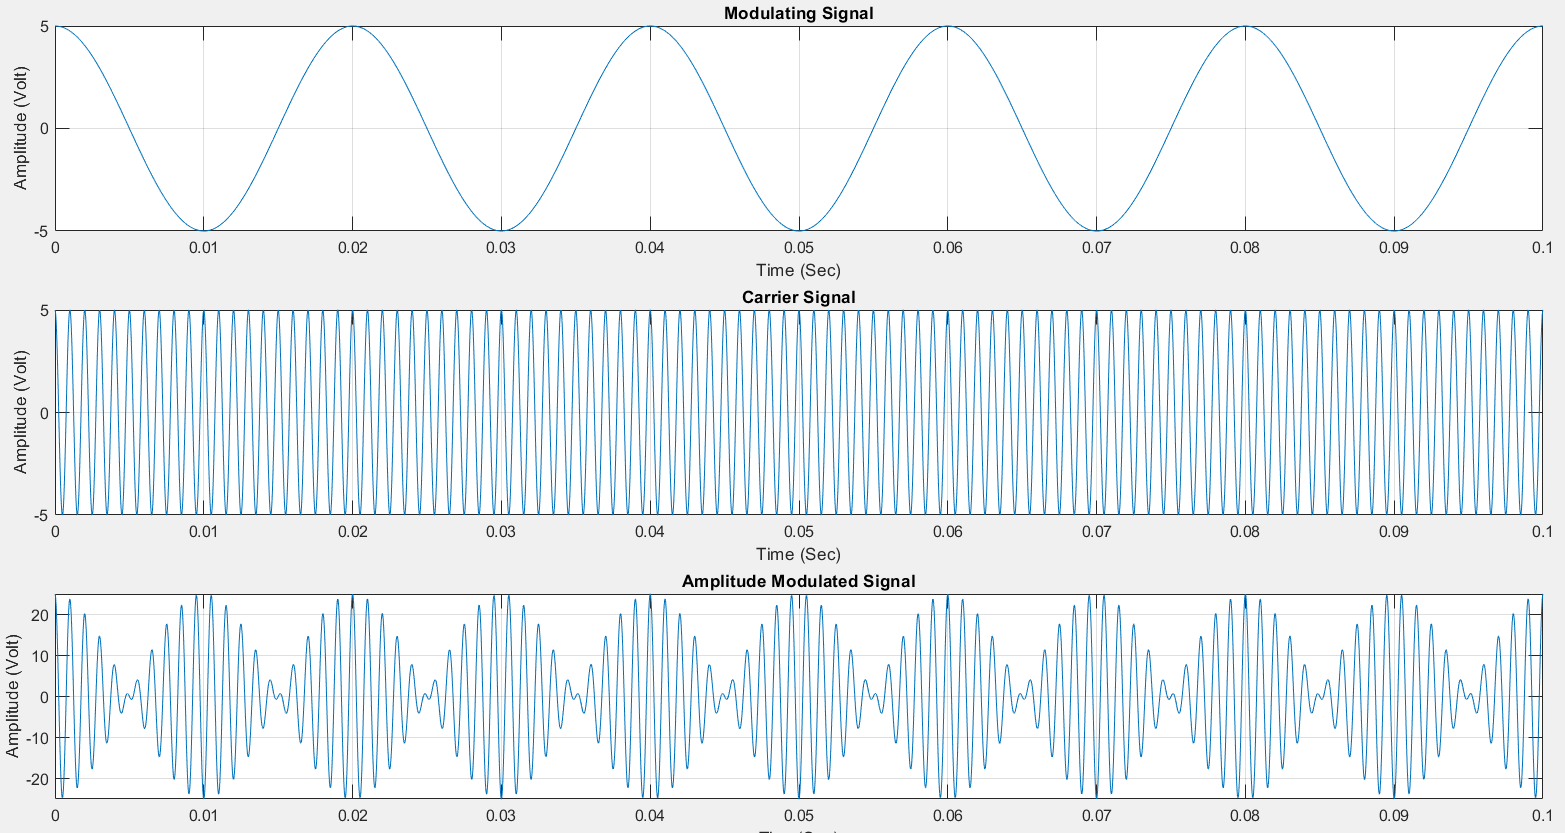
\includegraphics[width=.9\linewidth]{Figures/sim_dsb_sc.png}
          \caption{Simulated DSB-SC signal}
        \end{figure}
    \section{Discussion and Conclusion}
    The lab experiment dealt with the basic idea of amplitude modulation to get a modulated signal from a message and a carrier signal. The variation of Double side band- full carrier (DSB-FC) was observed based on the variation of the modulation index, $\mu$. During the lab experiment, message signal with frequnecy, $f_m=50$ Hz and carrier signal with frequency, $f_c=955$ Hz were generated using the signal generator. With the use of a balanced modulator, DSB-FC amplitude modulated signal was generated and visualized using the oscilloscope. The readings for the maximum and minimum voltages on the modulated signals were noted and the modulation index was calculated. To vary the index, the amplitude of carrier signal was varied, which is visible in the observations above. The modulation index obtained in each case is noted above. \\
    As a part of developing concept for DSB-FC and DSB-SC modulation, MATLAB script for generation of both the signals is also included in this report. As mentioned earlier, the modulation index is represented by the variable $m$, which is entered by the user. The generated DSB-FC signals for different conditions of modulation are included in the report. Likewise the DSB-SC signal generated by essentially suppressing the additional carrier portion in the modulated signal is also included in the report. The modulated signal in such condition includes only the product of the message and carrier signals.\\
    The need for DSB-SC signal is established by the unnecessary power and bandwidth loss in DSB-FC while transmitting the additional carrier portion in the signal. This lab allowed us to visualize the amplitude modulation in varying conditions of modulation index. Hence, the objectives of the lab experiment are fulfilled. 
\end{document}